\documentclass{standalone}

\AtBeginDocument{\renewcommand{\AtBeginDocument}[1]{}}
\usepackage{siunitx}

\usepackage{pgfplots}
\pgfplotsset{compat=newest}

\begin{document}
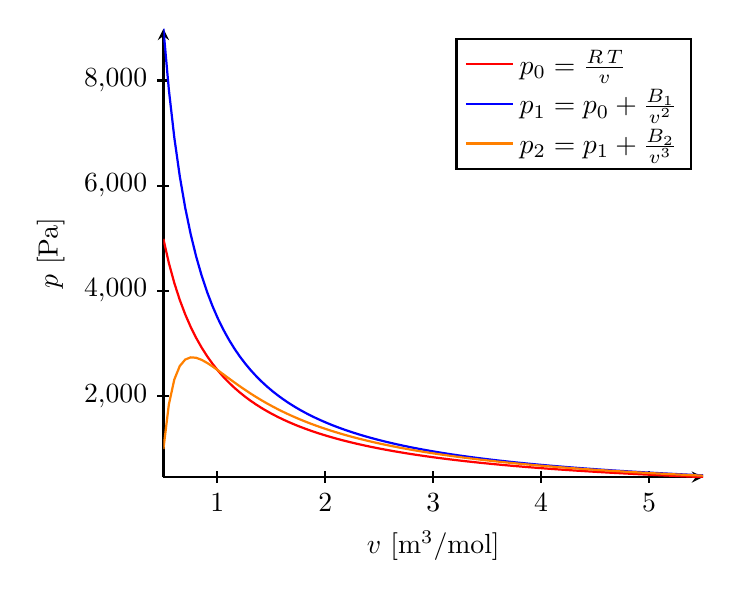
\begin{tikzpicture}

  \def\R{8.31}\def\T{300}
  \def\a{10^(-3)}\def\b{10^(-5)}

  %\def\Bone{(\b*\R*\T - \a)}
  %\def\Btwo{(\b^2*\R*\T - \a*\b + \a^2/(2*\R*\T))}
  \def\Bone{1000}
  \def\Btwo{-1000}

  \def\pzero{\R*\T/x}
  \def\pone{\pzero + \Bone/x^2}
  \def\ptwo{\pone + \Btwo/x^3}

  \begin{axis}[
    axis lines=left,
    samples=100,
    domain=0.5:5.5,
    xlabel={$v$ [\si{\meter\cubed\per\mol]}},
        ylabel={$p$ [\si{\pascal}]},
        every tick/.style={thick},
        thick]

    %p_0
    \addplot[color=red]{\pzero};
    \addlegendentry[right]{$p_0 = \frac{R \, T}{v}$}

    %p_1
    \addplot[color=blue]{\pone};
    \addlegendentry[right]{$p_1 = p_0 + \frac{B_1}{v^2}$}

    %p_2
    \addplot[color=orange]{\ptwo};
    \addlegendentry[right]{$p_2 = p_1 + \frac{B_2}{v^3}$}

  \end{axis}
\end{tikzpicture}
\end{document}